\section{Bounds for the Rendezvous Value}
With the existence and uniqueness being proven, it is a natural question to ask  which values $a(X,f)$ might take. To examine this we first require the following definition.

\begin{definition}
	Let $X$ be a compact connected Hausdorff space and $f: X\times X\to \R$ a continuous and symmetric function. We call 
	\[
	D(X,f):=\sup_{x,y}|f(x,y)|
	\]
	the \emph{diameter of $X$ with respect to $f$}.
\end{definition}
Note that this definition coincides with the usual one for metric spaces if $f$ is a metric on $X$.

The following result is due to Cleary, Morris and Yost \cite{cleary:numbers-of-shapes} and is a extension of a statement from Gross \cite{gross}.
\begin{theorem}\label{thm:metric-bounds}
	Let $(X,d)$ be a compact, connected, non-empty Hausdorff space. Let $n\in \N$. Then
	\begin{enumerate}
		\item $a(X,d^n)\geq 2^{-n}D(X,d^n)$ and 
		\item $a(X,d^n)< D(X,d^n)$ if $X$ is not a singleton.
	\end{enumerate}
\end{theorem}

\begin{proof}
	For the fist part, let $x_1$ and $x_2$ be diametrical points in $X$, i.e. $d(x_1,x_2)=D(X,d)$. Such exist, since $X$ is compact. By the Gross-Stadje-Theorem (\autoref{thm:gross-stadje}) we know that there is a $y\in X$ such that
	\begin{align*}
	a(X,d^n)&=\frac{1}{2}\left(d^n(x_1,y)+d^n(x_2,y)\right)\\
	&\geq\left(\frac{1}{2}d(x_1,y)+\frac{1}{2}d(x_2,y)\right)^n\\
	&\geq\left(\frac{1}{2}d(x_1,x_2)\right)^n=2^{-n}D(X,d^n).
	\end{align*}
	Thus, $a(X,d^n)\leq 2^{-n}D(X,d^n)$.
	
	For the second part, we only need to show that $a(X,d^n)\neq D(X,d^n)$. Assume for a contradiction that $a(X,d^n)=D(x,d^n)$ and let $x_1, x_2\in X$ be diametrical points. Then by \autoref{thm:gross-stadje} there is a $x_3\in X$ satisfying
	\[
	D(X,d^n)=a(X,d^n)=\frac{1}{2}\left(d^n(x_1,x_3)+d^n(x_2,x_3)\right).
	\]
	Since both $d^n(x_1,x_3)$ and $d^n(x_2,x_3)$ are bounded above by $D(X,d^n)$, this can only be the case for $d^n(x_1,x_3)=d^n(x_2,x_3)=D(X,d^n)$. Continuing this process inductively yields a sequence $(x_k)_{k\in \N}\in X$ such that $d^n(x_i,x_j)=D(X,d^n)\delta_{ij}$, where $\delta_{ij}$ denotes the Kronecker Delta. It is a sequence in a compact space that does not contain a convergent subsequence, which is not possible.
\end{proof}

Moving forward if will be inconvenient to state the results in terms of the rendezvous value and the diameter. We will simplify this as follows:
\begin{definition}
	We call 
	\[m(X,f):=\frac{a(X,f)}{D(X,f)}
	\]
	the \emph{dispersion constant}, sometimes also referred to as the \emph{magic number}.
\end{definition}

Obviously, the dispersion constant $m(X,f)$ can only take values in $[-1,1]$. We will see in the following section (see \autoref{thm:every-m-possible})that without further assumptions, this bound cannot be sharpened. However, we need some technical results first. 

\begin{definition}
	A space $E$ is called \emph{normal} provided that any two disjoint closed sets have disjoint neighborhoods.
\end{definition}

\begin{theorem}[Tietze extension theorem and Urysohn's lemma \cite{choquet:analysis}]\label{thm:tietze-urysohn}
	Let $E$ be a hausdorff space. Then the following statements are equivalent:
	\begin{enumerate}\renewcommand{\theenumi}{(\roman{enumi})}
	\item \label{equiv:normal} $E$ is normal.
	\item \label{equiv:Urysohn}For any two closed, non-empty, disjoint sets $A,B$, there is a continuous function $f:E\to [0,1]$ such that $f(A)=0$ and $f(B)=1$.
	\item\label{equiv:Tietze} For any closed set $A\subset E$ and continuous function $f: A\to [a,b]$, there exists $g: E\to [a,b]$ which is continuous and an extension of $f$.
	\end{enumerate}
\end{theorem}
The equivalence \ref{equiv:normal}$\Leftrightarrow$ \ref{equiv:Urysohn} is called Urysohn's lemma and \ref{equiv:normal}$\Leftrightarrow$\ref{equiv:Tietze} the Tietze extension theorem.
\begin{proof}
	%Without loss of generality, we may assume that $[a,b]=[-1,1]$. 
	The implications \ref{equiv:Urysohn}$\Rightarrow$\ref{equiv:normal} and \ref{equiv:Tietze}$\Rightarrow$\ref{equiv:Urysohn} are trivial.
	
\begin{description}[leftmargin=.25 cm]
	\item[\ref{equiv:normal}$\Rightarrow$\ref{equiv:Urysohn}:] Let $A$ and $B$ be two closed disjoint subsets of $E$. Since  $E$ is normal, there exists a open set $U$ such that
	\[
	A\subset U\subset \bar{U}\subset E\setminus B.
	\]
	Let $D$ be a countable, dense subset of $[0,1]$ and repeat above construction inductively (with $A$ replaced by $\bar{U}$), yielding a family of open sets $(U_t)_{t\in D}$ such that if $t<s$ we have
	\[
	A\subset U_t\subset \bar{U}_t\subset U_s\subset \bar{U}_s\subset E\setminus B.
	\]
	Now construct a function $f:X\to [0,1]$ by $f(x)=0$ if $x\in \bigcap_{t\in D} U_t$ and $f(x)=\sup\{t:x\not\in U_t\}$ otherwise. Note that
	\[
	f^{-1}([0,a))=\bigcup \{U_t: t<a\}
	\]
	and
	\[
	f^{-1}((a,1])=\bigcup \{E\setminus\bar{U}_t:t>a \}
	\]
	implies that $f$ is continuous.
	\item[\ref{equiv:Urysohn}$\Rightarrow$\ref{equiv:Tietze}:] Let $A$ be a closed subset of $E$ and $f:A\to [a,b]$ given. Note that we may replace $[0,1]$ in \ref{equiv:Urysohn} by any interval $[a,b]$. In particular, it is sufficient to prove \ref{equiv:Tietze} for the case of $[-1,1]$. Let $A_0=\{x\in A: f(x)\leq -\frac{1}{3}\}$ and $B_0=\{x\in A: f(x)\geq \frac{1}{3}\}$. By \ref{equiv:Urysohn} there is a continuous function $g_0: E\to [-\frac{1}{3},\frac{1}{3}]$ such that $g_0(A_0)=-\frac{1}{3}$ and $g_0(B_0)=\frac{1}{3}$. Let $f_1=f-g_0$ and repeat the procedure with $f_1$. Applying this process inductively yields a sequence
	\[
	f_n=f-(g_0+g_1+\dots+g_{n-1})=f-s_n
	\]
	such that $\|f_n\|_{\sup}\leq \left(\frac{2}{3}\right)^n$,
	 and $\|g_n\|_{\sup}\leq \frac{1}{3}\left(\frac{2}{3}\right)^n$. Therefore, $s_n$ converges uniformly to a function $g$ on $E$ which agrees with $f$ on $A$.\qedhere
\end{description}
\end{proof}

%\begin{theorem}[Tietze extension theorem and Urysoh\cite{munkres:topology}]
%	Let $X$ be a normal space; let $A$ be a closed subspace of $X$. Any continuous map of $A$ into the closed interval $[a,b]\subset \R$ may be extended to a continuous map of all of $X$ into $[a,b]$.
%\end{theorem}
%\begin{proof}
%	Let $f:A\to [a,b]$ be continuous. We will construct a sequence of functions $s_n: X\to [a,b]$ such that this sequence converges uniformly and such that the limit function coincides with $f$ on $A$.
%\end{proof}

The following statement ensures, that in our usual case, i.e. $X$ being a compact, connected, non-empty Hausdorff space, we may apply the Tietze extension theorem and the Urysohn lemma.
\begin{lemma}
	Every compact Hausdorff space is normal. 
\end{lemma}
The proof is due to Munkres \cite[p. 202]{munkres:topology}.
\begin{proof}
	We begin by showing that every compact hausdorff space $X$ is regular, i.e. given a closed set $A$ and a point $x\in X$ not in $A$, there exist disjoint neighborhoods of $A$ and $x$ respectively. Since $X$ is hausdorff, there are disjoint open sets $U_y$ of $y$ and $V_y$ of $x$. It is clear, that the $U_y$ are a open cover of $A$. Since $A$ is a closed subset of a compact space, $A$ is compact. Thus, there is a finite selection of points $(y_i)$ such that $U=\bigcup\limits_{i=1}^n U_{y_i}$ contains $A$. Since all $U_{y_i}$ are open, so is $U$. Similarly, $V=\bigcap\limits_{i=1}^n V_{y_i}$ is open as the intersection of finitely many open sets. Further, $U$ and $V$ are disjoint, proving regularity.
	
	We use a similar process to prove normality. Let $A$ and $B$ be disjoint closed subsets of $X$. Since $X$ is regular, for all $x\in B$ there are neighborhoods $U_x$ of $A$ and $V_x$ of $x$. Then the $V_x$ form a open cover of $B$. Since $B$ is compact as a closed subset of a compact space, there is a finite collection $(x_i)$ such that $V=\bigcup\limits_{i=1}^rV_{x_i}$ contains $B$. Define $U:=\bigcap\limits_{i=1}^rU_{x_i}$, then $U$ and $V$ are disjoint open neighborhoods of $A$ and $B$ respectively, proving regularity.
\end{proof}

We are now able to prove the following statement, which was formulated by Cleary and Morris \cite{cleary-morris}. However, the proof is based on the argument in \cite{cleary:numbers-of-shapes} by Cleary, Morris and Yost.
\begin{theorem}\label{thm:every-m-possible}
	Let $X$ be a compact, connected Hausdorff space with infinitely many points. Then for each real number $m\in[-1,1]$ there is a $f\in C_s(X,\R)$ such that $m(X,f)=m$.
\end{theorem}

\begin{proof}
	We will first examine the case of $m\geq 0$. Choose distinct points $a,b,c\in X$. Define
	\[
	S:=(X\times \{c\})\cup (\{c\}\times X)\cup \{(a,b)\}\cup \{(b,a)\}.
	\]
	Then $S$ is a closed subspace of the compact Hausdorff space $X\times X$. Define $g:S\to [0,1]$ as $g(x,c)=g(c,x)=\sqrt{m}$ for all $x\in X$ and $g(a,b)=g(b,a)=1$. Note, that $g$ is continuous.
	We now apply Tietze's extension theorem, which states that there is a continuous function $\theta: X\times X\to [0,1]$ such that $g(s)=\theta(s)$, for all $s\in S$. Now set $f$ to be the function from $X\times X$ to $[0,1]$ with $f(x,y)=\theta(x,y)\theta(y,x)$. Then $f$ is a continuous symmetric function with $f(x,c)=m$ for all $x\in X$. By considering the case $n=1$ and $x_1=c$, we immediately see from the definition of the rendezvous value that $a(X,f)=m$. Since $f(a,b)=1$ it is also clear that $D(X,f)=1$, yielding $m(X,f)=m$.
	
	In the case of $m<0$, we can construction an $f$ with $m(X,f)=-m$ analogously. Setting $f^\prime:=-f$ gives $m(X,f^\prime)=m$.
\end{proof}



%Beweis besser in numbers of shapes.

%\begin{definition}\cite{choquet:analysis}%completely regular
%	A space $E$ is called \emph{comletely regular} provided that for each $a\in E$ and neighborhood $U$ of $a$, there is a continuous map $f:E\to [0,1]$ such that $f(a)=0$ and $f(E\setminus U)=1$.
%\end{definition}



%\begin{lemma}[Urysohn's lemma, \cite{choquet:analysis}]
%	Let $E$ be a hausdorff space. Then $E$ is normal if and only if for any two closed, non-empty, disjoint sets $A,B$, there is a continuous function $f:E\to [0,1]$ such that $f(A)=0$ and $f(B)=1$.
%\end{lemma}


%\begin{lemma}
%	Every locally compact Hausdorff space is completely regular.
%\end{lemma}


%\begin{proof}
%	First, show that any compact hausdorff space is normal:
%\end{proof}

%However, we make a stronger statement if we restrict ourselves to the case of $(X,d)$ being a \emph{metric} space in addition to our other conditions.

The following result is due to Cleary and Morris \cite{cleary-morris} and shows that the rendezvous value is \emph{not} a topological invariant.

\begin{theorem}
	Let $X$ be a compact, connected, metrizable space with more than one point. Let $m\in [\frac{1}{2},1)$, then there exists a compatible metric $d$ such that $m(X,d)=m$.
\end{theorem}

\begin{proof}
	Let $\rho$ be a compatible metric such that $D(X,\rho)=1$. Choose $a,b\in X$ to be diametrical points and let $c\in X$ such that $\rho(a,c)=\frac{1}{2}$ ($c$ exists by virtue of the intermediate value theorem). Define a metric $d$ by
	\[
	d(x,y)=\min\left\{\rho(x,y),\min\left\{\frac{1}{2},\rho(c,x)\right\}+\min\left\{\frac{1}{2},\rho(c,y)\right\}\right\}.
	\] 
	We claim that this metric is equivalent to $\rho$ and $m(X,d)=\frac{1}{2}$. 
	
	To see that $d$ is a metric, it is easily verified that $d$ is symmetric and $d(x,y)=0$ if and only if $x=y$, since $\rho$ is a metric. The triangle inequality follows immediately from the following inequality:
	\[
	\rho(c,x)+\rho(c,y)\leq \rho(c,x)+\rho(c,y)-2\rho(c,z)=\rho(c,x)+\rho(c,z)+\rho(c,y)+\rho(c,z).
	\]
	
	In order to show that this metric is compatible, i.e. that $\rho$ induces the same topology as $d$, we only need to show
	\[
	\frac{1}{2}d(x,y)\leq\rho(x,y)\leq d(x,y)
	\]
	Here, the second inequality follows immediately from the definition of $\rho$.
	Suppose that $\rho(x,y)=\min\left\{\frac{1}{2},\rho(c,x)\right\}+\min\left\{\frac{1}{2},\rho(c,y)\right\}$, i.e. $\rho(x,y)\geq d(x,y)$.
	
	If $\min\left\{\frac{1}{2},\rho(c,x)\right\}=d(x,c)$ and $\min\left\{\frac{1}{2},\rho(c,y)\right\}=d(y,c)$, then $\rho(x,c)+\rho(y,c)=d(x,c)+d(y,c)\geq d(x,y)$. Thus, $\rho(x,y)=d(x,y)$. If $\min\left\{\frac{1}{2},\rho(c,x)\right\}\neq d(x,c)$, then $\min\left\{\frac{1}{2},\rho(c,x)\right\}=\frac{1}{2}\geq \frac{1}{2}d(x,y)$. Similarly, if $\min\left\{\frac{1}{2},\rho(c,y)\right\}\neq d(y,c)$, then $\rho(x,y)\geq \frac{1}{2}\geq \frac{1}{2}d(x,y)$. Hence, $\frac{1}{2}d(x,y)\leq \rho(x,y)\leq d(x,y)$.

	Now, since $d(x,c)\leq \frac{1}{2}$ for all $x\in X$ clearly $m(X,d)\leq \frac{1}{2}$. With the result from \autoref{thm:metric-bounds} we get $m(X,d)=\frac{1}{2}$.

		
	For $m>\frac{1}{2}$, define for $\lambda\geq 0$ metric
	\[
	d_\lambda:=\frac{(\lambda+1)d}{\lambda d+1}.
	\]
	We need to verify that $d_\lambda$ is in  fact a metric. Symmetry and identity of indiscernibles are obvious, since $d$ is a metric. The proof of the triangle inequality is not hard, but tedious:
	
	Firstly, notice that for $x,y,n\in \R$\[
	\frac{x+n}{y+n}-\frac{x}{y}=\frac{n(y-x)}{y(y+n)}.
	\]
	This enables us to find conditions under which $\frac{x+n}{y+n}\geq\frac{x}{y}$ (or $\leq$ respectively).
	Consider
	\begin{align*}
		\frac{(\lambda+1)d(x,z)}{\lambda d(x,z)+1}&+\frac{(\lambda+1)d(z,y)}{\lambda d(z,y)+1}=\frac{2\lambda(\lambda+1)d(z,y)d(z,x)+(\lambda+1)(d(x,z)+d(y,z)}{\lambda^2d(x,z)d(y,z)+\lambda(d(x,z)+d(y,z))+1}\\
		&\geq\frac{2\lambda(\lambda+1)d(z,y)d(z,x)+d(x,z)+d(z,y)+\lambda d(x,y)}{\lambda^2d(x,z)d(z,y)+\lambda d(x,y)+1}\\
		&\geq \frac{2\lambda(\lambda+1)d(z,x)d(z,y)+(\lambda+1)d(x,y)}{\lambda^2d(x,z)d(y,z)+\lambda d(x,y)+1}\\
		&\geq \frac{\lambda^2d(x,z)d(z,y)+(\lambda+1)d(x,y)}{\lambda^2d(x,z)d(z,y)+\lambda d(x,y)+1}\\
		&\geq \frac{(\lambda+1)d(x,y)}{\lambda d(x,y)+1}.
	\end{align*}
	
	Since $d_\lambda(a,b)=1$ for all $a,b\in X$ for which $d(x,y)=1$, we have $D(X,d_\lambda)=1$ for all $\lambda$. Further, if $x\neq y$, then $d_\lambda(x,y)\to 1$ as $\lambda\to \infty$. 
	
	We now claim that the dispersion constant $m(X,d_\lambda)$ depends continuously on $\lambda$. To see that, we only need to show that $d$ depends continuously on $\lambda$ with respect to the uniform topology on $C_S(X)$ and then apply Corollary \ref{cor:continuous}.
	We will prove this with a standard $\varepsilon$-$\delta$-proof:
	
	Let $\varepsilon>0$ and and $\lambda_0\geq 0$. Set 
	\[\delta:=\frac{\varepsilon}{2\cdot \sup\limits_{x,y\in X}(d^2(x,y)+d(x,y)}>0.\]
	Now, let $|\lambda-\lambda_0|<\delta$.
	Then 
	\begin{align*}
		|d_\lambda-d_{\lambda_0}|=&\left|\frac{(\lambda+1)d(x,y)}{\lambda d(x,y)+1}-\frac{(\lambda_0+1)d(x,y)}{\lambda_0 d(x,y)+1}\right|
		\\
		=&\left|\frac{(\lambda+1)\lambda_0d^2(x,y)+(\lambda+1)d(x,y)}{\lambda\lambda_0d^2(x,y)+\lambda d(x,y)+\lambda_0d(x,y)+1}\right.
		\\
		&\qquad\qquad -\left.\frac{(\lambda_0+1)\lambda d^2(x,y)+(\lambda_0+1)d(x,y)}{{\lambda\lambda_0d^2(x,y)+\lambda d(x,y)+\lambda_0d(x,y)+1}}\right|
		\\
		\leq&\frac{d^2(x,y)|\lambda_0-\lambda|+d(x,y)|\lambda-\lambda_0|}{|\lambda\lambda_0 d^2(x,y)+\lambda d(x,y)+\lambda_0 d(x,y)+1|}
		\\
		\leq& \frac{(d^2(x,y)+d(x,y))\delta}{\underset{>1}{\underbrace{|\lambda\lambda_0 d^2(x,y)+\lambda d(x,y)+\lambda_0 d(x,y)+1|}}}
		\\
		\leq &(d^2(x,y)+d(x,y))\delta.
	\end{align*}
	Therefore,
	\[
	\|d_\lambda-d_{\lambda_0}\|_{\infty}< \epsilon.
	\]
	
	Clearly $m(X,d_\lambda)\to 1$ as $\lambda\to \infty$. Since $m(X,d_0)=\frac{1}{2}$, the intermediate value theorem yields the existence of a $\lambda\in [0,\infty)$ with $m(X,d_\lambda)=m$.
\end{proof}


Stadje \cite{stadje} found a bound for compact convex subspaces of the euclidean 2-space. He further stated, that the same bound holds for higher dimensions. J. Strantzen \cite{strantzen} and E. Szekeres and G. Szekeres (according to Cleary, Morris and Yost \cite{cleary:numbers-of-shapes}, quoting private communication), however, independently proved that this is not correct. Stranzen gives the correct bound, which we will discuss after some preliminary work.

\begin{theorem}
	Let $d$ be the euclidean metric on $\R^2$ and $X\subset \R^2$ be a compact convex set. Then \[
	a(X,d)\leq \frac{1}{2}\sqrt{5-2\sqrt{3}}D(X,d).
	\]
\end{theorem}
\begin{proof}
	If $X$ consists of a single point, then the statement is trivial. Consider the case where $X$ consists of at least two points. Choose $x_1,x_2\in X$ to be diametrical and let $\frac{1}{2}(x_1+x_2)$ be the origin of a coordinate system as pictured below.
	
	\begin{centering}
	\begin{tikzpicture}
		\draw[->] (-5,0)->(5,0) node[right]{$t$};
		\draw[->] (0,-3)->(0,3) node[above]{$s$};
		\draw (4.33,0) arc[start angle=30, end angle=150, radius=5];%midpoint (0,-2.5)
		\draw[dashed] (5,-2.5) arc[start angle=0, end angle=180, radius=5];
		\draw[dashed] (-5,2.5) arc[start angle=180, end angle=360, radius=5];
		\draw (-4.33,0) arc[start angle=210, end angle=330, radius=5];
		\draw (-0.2,-2.5)  node[below]{$x_1$};
		\draw (-0.2,2.5) node[above]{$x_2$};
		\filldraw (-0,-2.5) circle (0.075);
		\filldraw (-0,2.5) circle (0.075);
		\filldraw (2.5,1.83) circle (.075) node[above]{$x_3$};
		\filldraw (-2.5,1.83) circle (.075) node[above]{$x_4$};
		\filldraw[pattern=north east lines] (0,2.5)--(2.5,1.83)--(0,-2.5)--(-2.5,1.83)--cycle;
	\end{tikzpicture}
	
	\end{centering}
	
	For the purpose of finding an upper bound for $a(X,d)$ we may restrict ourselves to dirac measures of points on the $t$-axis. Let $B((t,0),a)$ be the ball with center $(t,0)$ and radius $a$. Clearly, if $X\subset B((t,0),a)$ then $a\geq a(X,d)$, since \[\int\limits_X d(x,(t,0))\mu(\dx)\leq a\quad \forall \mu\in \M^1(X).\] 
	
	Let $(t^\prime,s^\prime)=\arg\max\limits_{(t,s)\in X}(|t|)$. Without loss of generality, we can assume $t^\prime,s^\prime>0$. Again, $X\subset B((t^\prime,s^\prime),D)$. The goal is now to choose $a$ such that $B(x_1,D)\cap B(x_2,D)\cap B((t^\prime,s^\prime))\subset B((t,0),a)$ for some $t$.
	
	Let $x_3$ and $x_4$ be the points on the upper arc which have the same $s$-coordinate and distance $D(X,d)$. A simple geometrical argument yields, that 
	\begin{align*}
	x_3&=\left(\frac{D(X,d)}{2},D(X,d)\cos\left(\frac{\pi}{6}\right)-\frac{D(X,d)}{2}\right)=\frac{D(X,d)}{2}(1,\sqrt{3}-1)\\
	x_4&=\frac{D(X,d)}{2}(-1,\sqrt{3}-1)
	\end{align*}
	
	The distance from $x_3$ (and $x_4$) to the origin is easily computed to be $\frac{D(X,d)}{2}\sqrt{5-2\sqrt{3}}$. The (filled, 2-dimensional) quadrangle spanned by $x_1, x_2,x_3,x_4$ (shaded in the picture above) cannot be contained in a ball with center on the $t$-axis and radius $a\leq \frac{D(X,d)}{2}\sqrt{5-2\sqrt{3}}$. Further, this radius suffices for all possible $(s^\prime,t^\prime)$ %TODO I dont understand the rest of the argument!!! By Symmetry?
	by symmetry. %todo is that true?
	A interactive GeoGebra worksheet to this is available on: \url{www.geogebra.org/u/janzwank}
\end{proof} %review frontier


To find the upper bound for the higher dimensional case, we fist need to investigate surfaces of smallest radius enclosing bounded subsets of $n$-dimensional euclidean space, following Blumenthal's approach \cite{blumenthal}. For this purpose, we need the following result from Helly \cite{helly} first.

\begin{lemma}\label{lem:helly}
	For any collection of closed convex subsets $\mathcal{K}:=\{K_i\}_{i\in I}$ of some $\R^n$ for which each subcollection $\{K_{i_1},\dots,K_{i_{n+1}}\}$ of $n+1$ sets has at least one common point, i.e. $\bigcap\limits_{k=1}^{n+1} K_{i_k}\neq \emptyset$, there exists a point in the intersection of all sets, i.e. $\bigcap\limits_{i\in I} K_i\neq \emptyset$.
\end{lemma}

\begin{proof}
	For $n=1$ this is easy to see. Note that in dimension one closed convex subsets of $\R^1$ are essentially line segments (whose endpoint might be $\pm\infty$). Each pair of two such line segments has at lest one common point. Let 
	\[
	a_i=\inf K_i \quad\text{and}\quad b_i=\sup K_i,
	\]
	then clearly 
	\[
	\sup a_i\leq \inf b_i.
	\]
	Thus, there exists a point $p\in \R^n$ with $p\in\bigcap\limits_{i\in I} K_i$.
	
	We will now apply a proof by induction. Suppose above statement holds for dimensional less than $n-1$ and for the special case of dimension $n$ for $|I|\leq p$ sets, where $p>n+1$ (the case $p=n+1$ is trivial).
	
	Let $K_1,\dots K_p$ be $p$ closed convex subsets of $\R^n$. Let $K$ be another closed convex subset such that $K_1,\dots,K_p,K$ satisfy the requirements of the lemma. Let $G=\bigcap_{i=1}^p K_i\neq \emptyset$. G itself is a closed convex subset of $\R^n$. Suppose for a contradiction that our statement is incorrect, then it must be possible to choose $K$ such that $K$ has a common point with each subcollection of $n$ sets of $K_1,\dots,K_p$, and simultaneously $K\cap G=\emptyset$. In this case there exists a hypersurface $H$ separating $G$ and $K$ with $H\cap G=H\cap K=\emptyset$. Now consider the intersections of each pairing of $n+1$ sets in $\mathcal{K}$. Then these sets all contain $G$ and at least one point of $K$. Thus, all such sets must have at least one common point with $H$. This means that for 
	\[
	k_{i}=K_{i}\cap H
	\]
	each collection of $n$ such $k_i$ has at least one common point in $H$. By induction hypothesis we have $\bigcap_{i\in I}k_i\neq 0$. But $\bigcap_{i\in I}k_i\subset G$ and thus we get a contradiction to $H\cap G=\emptyset$. Hence, $K$ and $G$ have at least one common point. This completes the proof for finitely many sets, i.e. $|\mathcal{K}|\neq \infty$.
	
	The statement for countably many sets follows by successively adding more sets and exploiting that all sets in $\mathcal{K}$ are closed. Now, consider the case of $I$ being uncountable. For this, choose any countable subset $N^\prime$ of $I$. Denote the (nonempty) set of common points as $G^\prime$. Let $r^\prime$ be its dimension. Let $r$ denote the smallest possible value of $r^\prime$.
	
	Further, each $G^\prime$ has a capacity %todo is this the correct word? German: Inhalt
	$V^\prime$. Let $V:=\inf V^\prime$, where the infimum is taken over all $G^\prime$ of dimension $r$.
	
	Let $N_1,N_2,\dots$ be a sequence of countable subsets of $I$, with common sets $G_1,G_2,\dots$ such that the corresponding sequence $V_1,V_2,\dots$ converges to $V$. Now, let $N=\bigcup_{k=1}^\infty N_k$. Then $N$ is again countable and the common sets $G$ has dimension $r$ and capacity $V$. We now claim that $G$ is contained in all sets in $\mathcal{K}$, for if it wasn't contained in some set $K\in \mathcal{K}$, then the sequence consisting of $K$ and $\{K_i\}_{i\in K}$ would yield a capacity less than $V$, which contradicts the definition of $V$.
\end{proof}

\begin{definition}
	Let $S_{n-1,r}$ denote the ($n-1$-dimensional) spherical surface (i.e. the boundary of the $n$-dimensional ball) of radius $r$ in $E_n$ (the euclidean $n$-space). A given spherical surface \emph{encloses} $M\subset E_n$ if $M$ is a subset of the closed ball whose boundary is given by $S_{n-1,r}$. If there exists a smallest radius $\rho(M)$ for which $S_{n-1,\rho(M)}$ encloses $M$, we call $\rho(M)$ the \emph{Chebyshev-out radius of $M$} and the center $c(M)\subset M$ of this sphere the \emph{Chebyshev center of $M$}. 
\end{definition}

The following lemma reduces the problem to the case of finitely many points.

\begin{lemma}\label{lem:blumenthal-lem1}
	If each set of $n+1$ points of a subset $M$ of $E_n$ is enclosable by $S_{n-1,r}$ of given radius $r$, then $M$ is itself enclosable by this $S_{n-1,r}$.
\end{lemma}
\begin{proof}
	Let $\overline{B^{(n)}(x,r)}$ denote the $n$-dimensional ball with radius $r$ and center $x$. Consider the family $\{\overline{B^{(n)}(x,r)}\}_{x\in M}$. Since each set of $n+1$ points of $M$ is enclosable by $S_{n-1,r}$ we see that each choice of $n+1$ balls has non-empty intersection. With a lemma of Helly (Lemma \ref{lem:helly}) 
	we find that there is a point $p$ common to all such balls. Thus, $M\subset \overline{B^{(n)}(p,r)}$.
\end{proof}

\begin{lemma}\label{lem:blumenthal-lem2}
	Let $P=\{p_1,\dots, p_{n+1}\}$ be a set of $n+1$ points of $E_n$ with diameter $D>0$. There exists a positive number $r$ such that $P$ is enclosable by $S_{n-1,r}$ and not enclosable by any $S_{n-1,r^\ast}$ with $r^\ast< r$. 
\end{lemma}
\begin{proof}
	This statement is an immediate consequence of $P$ being compact in $E_n$.
\end{proof}

\begin{lemma}\label{blumenthal-property1}
	In the situation of the previous lemma, the center $c$ of $S_{n-1,r}$ is a point of the simplex whose vertices are the points of $P$.
\end{lemma}

\begin{proof}
	Assume for a contradiction that $c$ is not contained in this simplex. Then a face of codimension one separates $c$ from the vertex opposite of this hyperplane. Since the spherical surface $S_{n-1,r^\ast}$, erected on the intersection of this hyperplane with $S_{n-1,r}$ (the center of this spherical surface is the orthogonal projection of $c$ on $x_n=0$) encloses $P$ with $r^\ast<r$, we get a contradiction. For $n=2$ this is depicted below.
\end{proof}

\begin{centering}
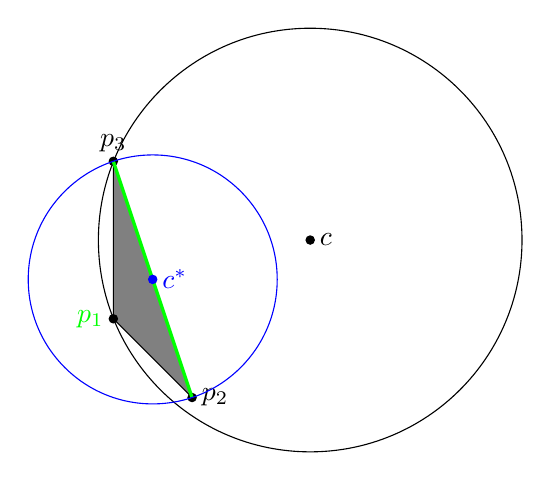
\begin{tikzpicture}
	\filldraw[fill=gray,draw=black] (0,0) node[left, green]{$p_1$}--(0,2)node[above]{$p_3$}--(1,-1) node[right]{$p_2$}--cycle;
	\filldraw (2.5,1) circle(1.5pt) node[right]{$c$};
	\filldraw (0,0) circle (1.5pt);
	\filldraw (0,2) circle (1.5pt);
	\filldraw (1,-1) circle (1.5pt);
	\draw (2.5,1) circle (2.69);
	\draw[green, very thick](0,2)--(1,-1);
	\filldraw[blue] (0.5,0.5) circle (1.5pt) node[right]{$c^\ast$};
	\draw[blue] (0.5,0.5) circle (1.581);
\end{tikzpicture}

\end{centering}

\begin{lemma}\label{blumenthal-property2}
	Let $P,c$ and $S_{n-1,r}$ as above. If a point of $P$ is not on $S_{n-1,r}$, then $c$ lies in the face of the simplex opposite this point.
\end{lemma}

\begin{proof}%todo i don't understand the notation! What is |S_{n-1,r}(p_j)|?
	Assume for a contradiction that there exists a point $p_j\in P$ which is not in $S_{n-1,r}$ and select a Cartesian coordinate system so that the $n-1$-dimensional hyperplane determined by the points $p_1,\dots, p_{j-1},p_{j+1},\dots, p_{n+1}$ have vanishing $n$-th coordinate $x_n$ and the $n$-th coordinate of $p_j$, denoted by $x_n^{(j)}$ is positive. The previous lemma implies that $c_n$ (the $n$-th coordinate of $c$) is positive.
	
	Let $0<t<\min\left\{\frac{|S_{n-1,r}(p_j)|}{2x_n^{(j)}},c_n\right\}$, where $S_{n-1,r}(x):={(x_1-c_1)^2+\dots+(x_n-c_n)^2}-r^2$. Consider $S_{n-1,r^\ast}$ satisfying the equation
	\[
	S_{n-1,r}+2tx_n=0
	\]
	
	The left-hand-side of this equation is always less or equal to zero for each of the points $p_1,\dots,p_{j-1},p_{j+1},\dots,p_{n+1}$ since $S_{n-1,r}$ encloses these points and each of them are in the plane $x_n=0$. Furthermore, we chose $t$ such that
	\[
	S_{n-1,r}(p_j)+2tx_n^{(j)}<S_{n-1,r}(p_j)+|S_{n-1,r}(p_j)|=0.
	\]
	Thus $S_{n-1,r^\ast}$ encloses all of the $n+1$ points of $P$. However, this is impossible, since $S_{n-1,r^\ast}$ is a linear combination of these loci, 
	and since $0<t<c_n$ the center $(c_1,c_2,\dots,c_{n-1},c_n-t)$ of $S_{n-1,r^\ast}$ is closer to the plane $x_n=0$ than it is to the center $c$ of $S_{n-1,r}$. Hence $r^\ast<r$ contradicting the minimality of $r$.
\end{proof}

\begin{lemma}\label{lem:blumenthal-lem3}
	Let $P$ be a set of $n+1$ points of $E_n$, not of $E_{n-1}$ of diameter $D$. If $S_{n-1,r}$ is an $(n-1)$-dimensional spherical surface of smallest radius $r$ enclosing $P$, then $r\leq D\sqrt{\frac{n}{2n+2}}$.
\end{lemma}

\begin{proof}
	Let $P_1, P_2,\dots, P_{n+1}$ be the vectors corresponding to the points $p_1,p_2,\dots,p_{n+1}$ of $P$ and let $C$ be the corresponding vector to the center $c$. By virtue of lemma \ref{blumenthal-property1} there exist $k_1,\dots,k_{n+1}\in\R^+_0$ with
	\begin{equation}\label{blumenthal-equation}
	\sum_{i=1}^{n+1}k_i=1\qquad\text{and}\qquad C=k_1P_1+k_2P_2+\cdots+k_{n+1}P_{n+1}
	\end{equation}
	Without loss of generality, we can assume $k_{n+1}\geq k_i$ for all $1\leq i\leq n+1$ by relabeling if necessary. Then $k_{n+1}>0$, thus $c$ is not contained in the face opposite of $p_{n+1}$ and by virtue of lemma \ref{blumenthal-property2} $p_{n+1}$ is on $S_{n-1,r}$.
	
	Since the constants $k_1,\dots, k_{n+1}$ are invariant under translation, we can translate the origin of the coordinate system to $p_{n+1}$ and have $P_i^T\cdot (2C-P_i)=0$ for each index $i$ with $k_i>0$, for if $k_i$ is positive then $p_i\in S_{n-1,r}$ by the same argument as above. Therefore for each such index $i$, we have $2P_i^T\cdot C=P_i^T\cdot P_i$.
	Since $k_i$ are either positive or zero, we see that the equality $2k_iP_i^T\cdot C=k_i(P_i^T\cdot P_i)$ holds for all indices $1\leq i\leq n+1$. We get
	\[
	\sum_{i=1}^{n}(k_iP_i^T)\cdot C=\frac{1}{2}\sum_{i=1}^nk_i(P_i^T\cdot P_i)=\frac{1}{2}\sum_{i=1}^{n}k_id_i^2,
	\]
	where $d_i$ denotes the length of $P_i$. With \eqref{blumenthal-equation} and $P_{n+1}=0$ we conclude 
	\[
	r^2=C^T\cdot C\leq \frac{1}{2}D^2\sum_{i=1}^{n}k_i.
	\]
	With $k_{n+1}\geq k_i$ for all $1\leq i\leq n+1$ and $\sum_{i=1}^{n}k_i=1-k_{n+1}$, so $k_{n+1}>\frac{1}{n+1}$ and we find \[
	r^2\leq \frac{n}{2(n+1)}D^2.
	\]
\end{proof}

\begin{theorem}\label{thm:blumenthal}
	Let $D$ be the diameter of the bounded set $M$ (containing more than a single point) of the $n$-dimensional euclidean space $E_n$. Then 
	\begin{enumerate}
		\item there exists a unique smallest spherical surface $S_{n-1,r}$ enclosing $M$ and
		\item $r\leq D\sqrt{\frac{n}{2(n+1)}}$.\label{statement:blumenthal2}
	\end{enumerate}
\end{theorem}

\begin{proof}
	We apply a inductive proof. The statement is trivial for $n=1$. Assume the assertion holds for every positive integer $k<n$. We consider two cases:
	\begin{description}
		\item[Case 1. $M\subset E_k$, $1\leq k<n$.] By induction hypothesis there exists a unique smallest $S_{k-1,r}$ enclosing $M$ and $r\leq D\sqrt{\frac{k}{2(k+1)}}<D\sqrt{\frac{n}{2(n+1)}}$, since $\frac{\mathrm{d}}{\mathrm{d}k}\frac{k}{2(k+1)}=\frac{1}{2(k+1)^2}>0$. It is clear that $S_{n-1,r}$ satisfies the requirements of the theorem.
		\item[Case 2. $M\not\subset E_k$\hspace{1ex}$\forall k<n$.] Consider the set $\{P\}$ of all sets of $n+1$ points of $M$ is not empty, and by lemma \ref{lem:blumenthal-lem2} there is a smallest $S_{n-1,r(P)}$ enclosing each $P$ of $\{P\}$. Let $r:=\sup\limits_{P\in \{P\}}r(P)$. Since $0<r(P)<D, P\in \{P\}, r$ is a positive (finite) number.
	\end{description}

\begin{myassertion*}
	The set $M$ is enclosable by $S_{n-1,r}$ and by no spherical surface of smaller radius.
\end{myassertion*}

Since $r\geq r(P)$ for all $P\subset M$ each set of $n+1$ points of $M$ is enclosable by $S_{n-1,r}$ and hence by lemma \ref{lem:blumenthal-lem1}, $M$ is enclosable by $S_{n-1,r^\ast}$. Assume $r^\ast<r$, then we get the existence of subset $P$ of $n+1$ points of $M$ with $r(P)>r^\ast$, by definition of $r$; thereby the smallest spherical surface enclosing this subset $P$ has a radius exceeding $r^\ast$. Thus, this subset and thereby $M$ is not enclosable by an $S_{n-1,r^\ast}$.

For the uniqueness part of the statement consider the following: Let $S_{n-1,r}(p)$ be a $(n-1)$-dimensional spherical surface of smallest radius $r$ enclosing $M$ with center $p$. Suppose that $S_{n-1,r}(q)$ is another spherical surface enclosing $M$. Then $M$ is contained in the intersection of the corresponding $n$-balls of radius $r$. Consequently, $M$ is enclosable by a $S_{n-1,r^\ast}$ with $r^\ast<r$. This proves uniqueness of both the radius as well as the center of $S_{n-1,r}$.

Statement \ref{statement:blumenthal2} follows from lemma \ref{lem:blumenthal-lem3}.
\end{proof}

With this preliminary work, we are now able to understand the proof for the following statement by Strantzen \cite{strantzen}.
%\begin{lemma}
%	Let $X$ be a bounded closed convex subset of $\R^n$ containing at least two points, and let $B$ be the closed ball of smallest radius such that $X\subset B$. If $b$ is the center of $B$ then $b\in X$.
%\end{lemma}
%\begin{proof}
%	This statement is an immediate consequence of lemma \ref{lem:blumenthal-lem1} and \ref{blumenthal-property1}.
%\end{proof}

\begin{theorem}
	Let $X$ be a bounded, closed, convex, non-empty subset of $\R^n$ and $D$ be the diameter of $X$. Then $a(X,d)\leq D\sqrt{\frac{n}{2n+2}}$.
\end{theorem}
\begin{proof}
	The statement is trivial if $X$ is just one point. If $X$ contains at least two points, we need only apply \autoref{thm:blumenthal} to find a ball $B$ of smallest radius $r\leq D\sqrt{\frac{n}{2(n+1)}}$. Let $b$ be the center of $B$. It is a immediate consequence of lemma \ref{lem:blumenthal-lem1} and lemma \ref{blumenthal-property1} that $b\in X$. Now apply the Gross-Stadje-Theorem (\autoref{thm:gross-stadje}) to the case of $n=1$ and $x_1=b$. Since $d(b,y)\leq r$ for all $y\in X$ we find $a(X,d)\leq r\leq D\sqrt{\frac{n}{2(n+1)}}$.
\end{proof}

Strantzen further proves that this bound is optimal by computing the rendezvous-value of the $k$-skeleton of a regular $n$-simplex of diameter $D$ to be
\[
a(\sigma^k,d)=\frac{D}{(n+1)\sqrt{2k+2}}((k+1)\sqrt{k}+(n-k)\sqrt{k+2}).
\]

For the case $k=n$ we see $a(\sigma^k,d)=d\sqrt{\frac{n}{(2n+2)}}$. Note that for $n\geq 4$ we have
\[
\sqrt{\frac{n}{2n+2}}\geq\frac{1}{2}\sqrt{5-2\sqrt{3}},
\]
proving that Stadje's bound is in fact erroneous for $n\geq 4$. For details, the reader is referred to Strantzen's paper \cite{strantzen}.


According to Cleary, Morris and Yost \cite{cleary:numbers-of-shapes} (quoting private communication) Esther and George Szekeres proved the following closely related result.

\begin{theorem}
	Let $X$ be a compact, convex subset of some normed space, with $d$ being the metric given by the norm. Then $a(X,d)=\rho(X)$, where $\rho(X)$ is the Chebyshev-out radius.
\end{theorem}

\begin{proof}
	Let $c(X)\in X$ be the Chebyshev center of $X$. Following the same logic as in the previous statement, we see $a(X,d)\leq\rho(X)$. To see the other inequality, choose $x_1,\dots,x_n\in X$ and define
	\[
	\Theta\colon X\to \R,\quad x\mapsto \frac{1}{n}\sum_{i=1}^nd(x,d_i).
	\]
	Since $X$ is connected, we only need to show $\Theta(x)\geq \rho(X)$ for some $x\in X$.
	
	Let $x_0=\frac{1}{n}\sum_{i=1}^{n}x_i\in X$, and choose $y\in X$ such that $d(y,x_0)\geq \rho(X)$. The existence of such $y$ follows form the definition of $\rho(X)$. Then
	\[
	\rho(X)\leq \|c-y\|\leq\frac{1}{n}\sum_{i=1}^{n}\|x_i-y\|=\Theta(y).\qedhere
	\]
\end{proof}

In general there is no inequality relation for subsets in the sense of $a(X,d)\stackrel{\leq}{\geq}a(Y,d)$ whenever $X\subset Y$. However, the following result due to Yost \cite{yost} holds true.

\begin{theorem}
	Let $X$ be a compact, connected, non-empty subset of a normed space. Let $Y$ be a closed, connected subset of $X$, and suppose that the convex hull of $Y$ contains $X$. Then $m(X,d)\leq m(Y,d)$, where $d$ is the metric induced by the norm.
\end{theorem}

\begin{proof}
	Since $Y\subset X\subset \mathrm{conv}(Y)$ it is clear that $D(X,d)=D(Y,d)$. Thus, we only need to show $a(X,d)\leq a(Y,d)$. Let $F$ denote any finite collection of points $x_1,\dots,x_n$ ($n\in \N$) in $Y$ (and therefore in $X$). Then by the Gross-Stadje-Theorem (\autoref{thm:gross-stadje}) there exists $x\in X$ satisfying
	\[
	a(X,d)=\frac{1}{n}\sum_{i=1}^{n}d(x_i,x).
	\]
	Since $X\subset \mathrm{conv}(Y)$ there exist $\lambda_1,\dots,\lambda_k\in \R_0^+, \sum_{j=1}^{k}\lambda_j=1$  and $y_1,\dots y_k\in Y$ with $x=\sum_{j=1}^{k}\lambda_j y_j$.
	Thus,
	\[
	a(X,d)=\frac{1}{n}\sum_{i=1}^n d\left(\sum_{j=1}^k y_j,x_i\right)\leq\sum_{j=1}^k\frac{\lambda_j}{n}\sum_{i=1}^n d(y_j,x_i).
	\]
	It is now clear %todo how clear is that?
	 that there is at least one $j$ with $a(X,d)\leq \frac{1}{n}\sum_{i=1}^n d(y_j,x_i)$ and therefore $a(X,d)\leq a(Y,d)$.
\end{proof}

The following result is an immediate consequence of this statement and due to Nickolas and Yost \cite{nickolas-yost:euclidean}

\begin{theorem}
	Let $X$ be a compact connected subset of $\R^n$. Then 
	\[m(X,d)\leq \sqrt{\frac{2n}{n+1}}a(S^{n-1},d),\]
	 %$m(X,d)\leq\frac{\Gamma\left(\frac{n}{2}\right)^2 2^{n-2}\sqrt{2n}}{\Gamma\left(n-\frac{1}{2}\right)\sqrt{(n+1)\pi}}$, 
	where $d$ denotes the euclidean metric.
\end{theorem}

\begin{proof}
	Without loss of generality, assume that $D(X,d)=1$. \autoref{thm:blumenthal} implies that $X\subset \mathrm{conv}(S^{n-1}_{\rho})$, where $\rho(X)$ denotes the Chebyshev-out radius and thus $\rho(X)\leq \sqrt{\frac{n}{2(n+1)}}$. With the result from the previous theorem we see
	$a(X,d)\leq\sqrt{\frac{2n}{n+1}}a(S^{n-1})$.
\end{proof}
In the next chapter we will discuss the computation of the rendezvous value of several spaces, including spheres.